\documentclass[aspectratio=169]{beamer}
\usepackage[utf8]{inputenc}
\usepackage[T1]{fontenc}
\usepackage{lmodern}
\usepackage{upquote}
\usepackage{amsmath}
\usepackage[copyright]{ccicons}
\usepackage{svg}
\usepackage{array}
\usepackage{booktabs}
\usepackage{textcomp}
\usepackage{subcaption}

\usepackage{tikz}
\usetikzlibrary{shapes.geometric, arrows, shapes.symbols, shadows, patterns}

\tikzstyle{start} = [rectangle, draw, text centered, rounded corners, align=center, minimum height=2em]
\tikzstyle{process} = [rectangle, draw, text centered, minimum height=2em]
\tikzstyle{data}=[trapezium, draw, text centered, trapezium left angle=60, trapezium right angle=120, minimum height=2em]
\tikzstyle{connector} = [draw, -latex']
\tikzstyle{cloud} = [cloud, draw, text centered, cloud puffs=10, cloud ignores aspect, minimum height=2em]
\tikzset{
  multidocument/.style={
    shape=tape,
    draw,
    fill=white,
    outer sep=3pt,
    tape bend top=none,
    double copy shadow},
  singledocument/.style={
    shape=tape,
    draw,
    fill=white,
    tape bend top=none},
  database/.style={
    cylinder,
    shape border rotate=90,
    aspect=0.1,
    align=center,
    draw}
}

\usepackage{float}

\usetheme{Boadilla}

\title[ForecastBench]{ForecastBench: A Dynamic Benchmark of AI Forecasting Capabilities}
\author[ForecastBench Team]{Ezra Karger\inst{1,2} \and Houtan Bastani\inst{1} \and Chen Yueh-Han\inst{3}\\\and Zachary Jacobs\inst{1} \and Danny Halawi\inst{4} \and Fred Zhang\inst{4} \and Philip E. Tetlock\inst{1,5}}
\institute[]{
  \inst{1} Forecasting Research Institute
  \inst{2} Federal Reserve Bank of Chicago
  \inst{3} New York University\\
  \inst{4} University of California, Berkeley
  \inst{5} University of Pennsylvania
}
\date[ICLR 2025]{ICLR 2025: April 24-28}

\AtBeginSection[]
{
  \begin{frame}
    \frametitle{Outline}
    \tableofcontents[currentsection]
  \end{frame}
}

\begin{document}

\begin{frame}
  \titlepage
\end{frame}

%\begin{frame}
%  \frametitle{Outline}
%  \tableofcontents
%\end{frame}

\section{A dynamic forecasting benchmark}

\begin{frame}
  \frametitle{Motivation}
  \begin{itemize}
  \item Forecasting is important and useful
    \begin{itemize}
    \item Evolution of a pandemic
    \item Economic indicators
    \item Geopolitical events
    \item ...
    \end{itemize}
  \item Human forecasting is time-consuming and expensive $\rightarrow$ LLM forecasters
    \begin{itemize}
    \item When will LLMs forecast as well as humans?
    \end{itemize}
  \item Previous forecasting benchmarks have been static
    \begin{itemize}
    \item Made obsolete once training cutoffs are after question resolution dates
    \item Knowledge cutoffs are imprecise
    \item Risk test set contamination
    \end{itemize}
  \end{itemize}
\end{frame}


\begin{frame}
  \frametitle{ForecastBench}
  \begin{itemize}
  \item Continuously updated with questions about future events $\rightarrow$ immune to look-ahead bias
  \item Periodic surveys of the general public and superforecasters $\rightarrow$ human comparison
  \item Fully automated benchmark with open source codebase
  \item Publicly available leaderboards updated nightly
  \item Datasets released regularly
    \begin{itemize}
    \item forecast questions
    \item forecasts by LLMs and humans, with rationales
    \item resolutions
    \end{itemize}
  \item Will be maintained at least until mid-2027 thanks to a grant from \href{https://www.openphilanthropy.org/}{Open Philanthropy}!
    \begin{block}{Links}
      \begin{itemize}
      \item Benchmark: \href{https://www.forecastbench.org/}{https://www.forecastbench.org}
      \item Code (MIT License): \href{https://github.com/forecastingresearch/forecastbench}{https://github.com/forecastingresearch/forecastbench}
      \item Data (CC-BY-SA-4.0 License):
        \begin{itemize}
        \item \href{https://github.com/forecastingresearch/forecastbench-datasets}{https://github.com/forecastingresearch/forecastbench-datasets}
        \item \href{https://huggingface.co/datasets/forecastingresearch/forecastbench-datasets}{https://huggingface.co/datasets/forecastingresearch/forecastbench-datasets}
        \end{itemize}
      \end{itemize}
    \end{block}
  \end{itemize}
\end{frame}


\section{Automated system}

\begin{frame}
  \frametitle{Automated System}
  Our automated system manages the benchmark, from updating the question bank, to generating and releasing question sets, to resolving forecasts and updating the leaderboard.
  \begin{itemize}
  \item \textbf{Question Bank}: updated nightly
  \item \textbf{Question Sets}: generated every 2 weeks
  \item \textbf{Eliciting Forecasts}: every 2 weeks from LLMs, periodically from the general public and superforecasters
  \item \textbf{Leaderboard}: updated nightly
  \end{itemize}
\end{frame}




\begin{frame}
  \frametitle{Question Bank}
  The Question Bank stores all questions to sample from. There are 2 types of questions:
  \begin{enumerate}
  \item \textbf{Market questions}: pulled from 4 forecasting platforms: Manifold, Metaculus, Polymarket, and the RAND Forecasting Initiative.
    \item \textbf{Dataset questions}: generated from 5 datasets: ACLED, DBnomics, FRED, Wikipedia, and Yahoo! Finance.
  \end{enumerate}
\begin{figure}[htb]
  \centering

    \begin{tikzpicture}[node distance=1.5cm and 2cm]
      % Define nodes using positioning
      \node (start) [start] at (-0.3,0) {Daily, \texttt{0:00} UTC};
      \node (questions) [process, right=of start] {Update Questions};
      \node (question_files_top) [multidocument, outer sep=4.2pt, below=of questions] {Question Files};
      \node (question_files_bottom) [multidocument, outer sep=2.4pt, below=of questions] {Question Files};
      \node (resolutions) [process, right=of questions, xshift=1cm] {Update Resolutions};
      \node (resolution_files_top) [multidocument, outer sep=4.2pt, below=of resolutions] {Resolution Files};
      \node (resolution_files_bottom) [multidocument, outer sep=2.4pt, below=of resolutions] {Resolution Files};
      \node (metadata) [process, right=of resolutions, xshift=1cm] {Update Metadata};
      \node (metadata_file) [singledocument, below=of metadata] {Metadata File};
      \node (metadata_file_outer) [singledocument, outer sep=2.4pt, below=of metadata] {Metadata File};
      \node (question_bank) [database, below=of resolution_files_bottom] {Question\\Bank};

      % Draw connectors
      \draw [connector] (start) -- (questions);
      \draw [connector] (questions.south) -- ([yshift=3.8mm]question_files_top.north);
      \draw [connector] (questions) -- (resolutions);
      \draw [connector] (resolutions.south) -- ([yshift=3.8mm]resolution_files_top.north);
      \draw [connector] (resolutions) -- (metadata);
      \draw [connector] (metadata) -- (metadata_file);
      \draw [connector] (metadata_file_outer.south) -- (question_bank.east);
      \draw [connector] (resolution_files_bottom.south) -- (question_bank.north);
      \draw [connector] (question_files_bottom.south) -- (question_bank.west);
    \end{tikzpicture}%

\end{figure}



%% \begin{figure}[htb]
%%   \centering
%%   \resizebox{0.9\columnwidth}{!}{%
%%     \begin{tikzpicture}[node distance=1.5cm and 2cm]
%%       % Define nodes using positioning
%%       \node (start) [start] at (-0.3,0) {Daily, \texttt{0:00} UTC};
%%       \node (questions) [process, right=of start] {Update Questions};
%%       \node (question_files_top) [multidocument, outer sep=4.2pt, below=of questions] {Question Files};
%%       \node (question_files_bottom) [multidocument, outer sep=2.4pt, below=of questions] {Question Files};
%%       \node (resolutions) [process, right=of questions, xshift=1cm] {Update Resolutions};
%%       \node (resolution_files_top) [multidocument, outer sep=4.2pt, below=of resolutions] {Resolution Files};
%%       \node (resolution_files_bottom) [multidocument, outer sep=2.4pt, below=of resolutions] {Resolution Files};
%%       \node (metadata) [process, right=of resolutions, xshift=1cm] {Update Metadata};
%%       \node (metadata_file) [singledocument, below=of metadata] {Metadata File};
%%       \node (metadata_file_outer) [singledocument, outer sep=2.4pt, below=of metadata] {Metadata File};
%%       \node (question_bank) [database, below=of resolution_files_bottom, yshift=-1cm] {Question\\Bank};

%%       % Draw connectors
%%       \draw [connector] (start) -- (questions);
%%       \draw [connector] (questions) -- (question_files_top);
%%       \draw [connector] (questions) -- (resolutions);
%%       \draw [connector] (resolutions) -- (resolution_files_top.north);
%%       \draw [connector] (resolutions) -- (metadata);
%%       \draw [connector] (metadata) -- (metadata_file);
%%       \draw [connector] (metadata_file_outer.south) -- (question_bank.east);
%%       \draw [connector] (resolution_files_bottom.south) -- (question_bank.north);
%%       \draw [connector] (question_files_bottom.south) -- (question_bank.west);
%%     \end{tikzpicture}%
%%   }
%% \end{figure}


%% \begin{figure}[htb]
%%   \centering
%%   \resizebox{0.9\columnwidth}{!}{%
%% \begin{tikzpicture}
%% \node (start) [start] at (-0.3,0) {Daily, \texttt{0:00} UTC};
%% \node (questions) [process] at (3,0) {Update Questions};
%% \node (question_files_outer_sep_top) [multidocument,outer sep=4.2pt] at (3,-1.12) {Question Files};
%% \node (question_files_outer_sep_bottom) [multidocument,outer sep=2.4pt] at (3,-1.12) {Question Files};
%% \node (resolutions) [process] at (6.5,0) {Update Resolutions};
%% \node (resolution_files_outer_sep_top) [multidocument,outer sep=4.2pt] at (6.5,-1.1) {Resolution Files};
%% \node (resolution_files_outer_sep_bottom) [multidocument,outer sep=2.4pt] at (6.5,-1.1) {Resolution Files};
%% \node (metadata) [process] at (10,0) {Update Metadata};
%% \node (metadata_file) [singledocument] at (10,-0.95) {Metadata File};
%% \node (metadata_file_outer_sep) [singledocument,outer sep=2.4pt] at (10,-0.95) {Metadata File};
%% \node (question_bank) [database] at (6.5,-2.5) {Question\\Bank};
%% \draw [connector] (start) -- (questions);
%% \draw [connector] (questions) -- (question_files_outer_sep_top);
%% \draw [connector] (questions) -- (resolutions);
%% \draw [connector] (resolutions) -- (resolution_files_outer_sep_top);
%% \draw [connector] (resolutions) -- (metadata);
%% \draw [connector] (metadata) -- (metadata_file);
%% \draw [connector] (metadata_file_outer_sep.south) --  (question_bank.east) ;
%% \draw [connector] (resolution_files_outer_sep_bottom.south) --  (question_bank.north) ;
%% \draw [connector] (question_files_outer_sep_bottom.south) --  (question_bank.west) ;
%%     \end{tikzpicture}}
%% \end{figure}

\end{frame}


\begin{frame}
  \frametitle{Question Sets}
  Every two weeks we sample 1,000 questions from the Question Bank to create the LLM Question Set.
  \begin{itemize}
  \item 500 standard questions: 250 market and 250 dataset questions.
  \item 500 \textit{combination} questions: 250 market and 250 dataset questions.
    \begin{itemize}
      \item Each combination question is just a pair of standard questions from the same source
      \item We ask for forecasts on the Boolean combinations of these questions: $P(Q1\cap Q2)$, $P(\neg Q1\cap Q2)$, $P(Q1\cap \neg Q2)$, and $P(\neg Q1\cap \neg Q2)$
    \end{itemize}
  \end{itemize}

  We sample 200 questions from the LLM Question Set to create the Human Question Set.
  \begin{itemize}
  \item 200 standard questions: 100 market and 100 dataset questions.
  \item No combination questions. Their combination forecasts are generated by treating $Q1$ and $Q2$ as independent, putting them at a disadvantage for these forecasts.
  \end{itemize}

\end{frame}

\begin{frame}
  \frametitle{Eliciting forecasts (1/2)}
  \begin{figure}[htb]
  \centering
  \resizebox{0.6\textwidth}{!}{%
  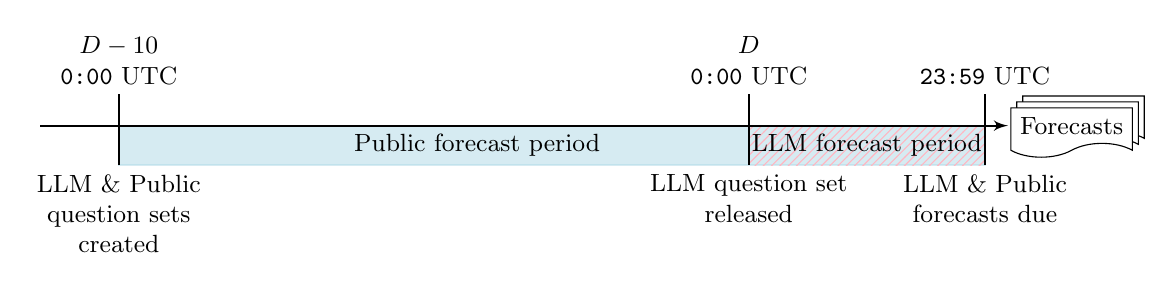
\begin{tikzpicture}[font=\small]
  \definecolor{lightblue}{RGB}{173, 216, 230}
  \definecolor{lightpink}{RGB}{255, 182, 193}

  \node (forecasts) [multidocument,outer sep=1pt] at (13.1,0) {Forecasts};

  \draw[fill=lightblue,draw=lightblue,opacity=0.5] (1, 0) rectangle (12, -0.5);
  \node[align=center] at (5.55, -0.25) {Public forecast period};

  \begin{scope}
    \path[fill=lightpink, pattern=north east lines, pattern color=lightpink] (9, 0) rectangle (12, -0.5);
  \end{scope}
  \node[align=center] at (10.5, -0.25) {LLM forecast period};

  % Main timeline
  \draw[thick, -{>[scale=1]},-latex'] (0, 0) -- (forecasts.west);

  % D-7
  \draw[thick] (1, -0.5) -- (1, 0.4);
  \node[below, align=center] at (1, -0.5) {LLM \& Public\\question sets\\created};
  \node[above, align=center] at (1, 0.4) {$D-10$\\\texttt{0:00} UTC};

  % D
  \draw[thick] (9, -0.5) -- (9, 0.4);
  \node[below, align=center] at (9, -0.5) {LLM question set\\ released};
  \node[above, align=center] at (9, 0.4) {$D$\\\texttt{0:00} UTC};

  % D
  \draw[thick] (12, -0.5) -- (12, 0.4);
  \node[below, align=center] at (12, -0.5) {LLM \& Public\\forecasts due};
  \node[above, align=center] at (12, 0.4) {\texttt{23:59} UTC};
\end{tikzpicture}}
   \caption{Timeline from question set generation to forecast due date, $D$.}

\end{figure}

  \begin{itemize}
  \item LLMs
    \begin{itemize}
    \item Forecast all 1,000 questions in the Question Set within 24 hours
    \item 17 models including GPT-4o, Claude Sonnet 3.5, Gemini 1.5 Pro, Qwen1.5 110B Chat, ...
    \item Prompting strategies: zero-shot, scratchpad, scratchpad with retrieval (i.e., news)
      \begin{itemize}
      \item For market questions, with or without crowd forecasts provided (what we term ``freeze values'')
      \end{itemize}
    \end{itemize}
  \item General public and superforecasters
    \begin{itemize}
    \item Forecast 200 questions sampled from the Question Set
    \item Surveys take 10 days to run
    \end{itemize}
  \end{itemize}
\end{frame}


\begin{frame}
  \frametitle{Eliciting forecasts (2/2): Forecast Sets}
  Forecasts are returned in \textbf{Forecast sets}. Each question requires a different number of forecasts to be produced.\\\ \\
  \resizebox{\textwidth}{!}{%
    \begin{tabular}{l p{8cm} c}
      \textbf{Question Type} & \textbf{Users forecast\ldots} & \textbf{\textnumero\ of Forecasts} \\ \hline
      Standard market questions & \ldots the final outcome & 1  \\ \hline
      Combination market questions & \ldots the final outcome for all Boolean combinations of the questions & 4  \\ \hline
      Standard dataset questions & \ldots the outcome $n$ days in the future, where $n \in N, N=\{7,30,90,180,365,1095,1825,3650\}$ & 8  \\ \hline
      Combination dataset questions & \ldots the outcome for all Boolean combinations of the questions at all forecast horizons in $N$ & 32  \\ \hline
    \end{tabular}%
  }

  \ \\$\Rightarrow$ for each Question Set, LLMs provide approximately $11,250$ forecasts in the corresponding Forecast Set: $250\times (1+4+8+32)$.
\end{frame}




\begin{frame}
  \frametitle{Leaderboard}
  The forecast sets produced bi-weekly are resolved every night and the leaderboard is updated.
  \begin{itemize}
  \item Market questions are scored against the crowd forecast until resolution, when they're scored against ground truth.
  \item Dataset questions are resolved against ground truth as datasets are updated and revised.
  \end{itemize}

\end{frame}


\section{Results}


\begin{frame}[fragile=singleslide]
  \frametitle{LLM/Human Leaderboard (top 10)}
  \begin{table}[ht!]
\centering
\tiny
\resizebox{0.75\columnwidth}{!}{%
\begin{tabular}{@{}l l l >{\centering\arraybackslash}m{2cm} >{\centering\arraybackslash}m{2cm} >{\centering\arraybackslash}m{2cm}@{}}
\toprule
Model & \begin{tabular}[c]{@{}l@{}}Information\\ provided\end{tabular} & Prompt & \begin{tabular}[c]{@{}l@{}}Dataset\\($N$=422)\end{tabular} & \begin{tabular}[c]{@{}l@{}}Market\\($N$=76)\end{tabular} & \begin{tabular}[c]{@{}l@{}}Overall\\($N$=498)\end{tabular} \\
\midrule
Superforecaster median forecast & -- & -- & 0.118 & 0.074 & 0.096 \\
Public median forecast           & -- & -- & 0.153 & 0.089 & 0.121 \\
Claude-3-5-Sonnet-20240620       & Freeze values & Scratchpad & 0.138 & 0.107 & 0.122 \\
Claude-3-5-Sonnet-20240620       & News with freeze values & Scratchpad & 0.142 & 0.112 & 0.127 \\
GPT-4-Turbo-2024-04-09          & Freeze values & Zero shot  & 0.162 & 0.095 & 0.128 \\
Claude-3-5-Sonnet-20240620       & Freeze values & Zero shot  & 0.145 & 0.117 & 0.131 \\
GPT-4                          & Freeze values & Zero shot  & 0.167 & 0.096 & 0.132 \\
GPT-4o                         & News with freeze values & Scratchpad & 0.162 & 0.105 & 0.133 \\
Claude-3-5-Sonnet-20240620       & -- & Scratchpad & 0.138 & 0.133 & 0.136 \\
GPT-4o                         & Freeze values & Scratchpad & 0.161 & 0.113 & 0.137 \\
\bottomrule
\end{tabular}
}
\end{table}

\end{frame}


\begin{frame}[fragile=singleslide]
  \frametitle{LLM Leaderboard (top 10)}
  \begin{table}[ht!]
\centering
\resizebox{\textwidth}{!} {%
\Large
\begin{tabular}{@{}l l l l >{\centering\arraybackslash}m{2cm} >{\centering\arraybackslash}m{2cm} >{\centering\arraybackslash}m{2cm} >{\centering\arraybackslash}m{3cm} >{\centering\arraybackslash}m{2cm} >{\centering\arraybackslash}m{2cm}@{}}
\toprule
& & & & \multicolumn{3}{c}{Brier Score $\downarrow$} \\ \cmidrule(lr){5-7}
Model & Organization & \begin{tabular}[c]{@{}l@{}}Information\\ provided\end{tabular} & Prompt & \begin{tabular}[c]{@{}l@{}}Dataset\\($N$=5,492)\end{tabular} & \begin{tabular}[c]{@{}l@{}}Market\\($N$=897)\end{tabular} & \begin{tabular}[c]{@{}l@{}}Overall\\($N$=6,389)\end{tabular} & \begin{tabular}[c]{@{}l@{}}Confidence\\ Interval\end{tabular} & \begin{tabular}[c]{@{}l@{}}Pairwise\\$p$-value\\comparing\\to No. 1\end{tabular} & \begin{tabular}[c]{@{}l@{}}Pct. more \\accurate\\ than No. 1\end{tabular} \\
\midrule
Claude-3-5-Sonnet-20240620 & Anthropic & Freeze values & Scratchpad & 0.169 & 0.078 & 0.123 & [0.117, 0.129] & -- & 0\% \\
GPT-4-Turbo-2024-04-09 & OpenAI & Freeze values & Scratchpad & 0.172 & 0.080 & 0.126 & [0.120, 0.132] & 0.096 & 43\% \\
GPT-4o & OpenAI & Freeze values & Scratchpad & 0.186 & 0.069 & 0.128 & [0.122, 0.133] & <0.01 & 43\% \\
Gemini-1.5-Pro & Google & Freeze values & Scratchpad & 0.162 & 0.106 & 0.134 & [0.128, 0.139] & <0.001 & 35\% \\
GPT-4o & OpenAI & News with freeze values & Scratchpad & 0.190 & 0.084 & 0.137 & [0.131, 0.143] & <0.001 & 39\% \\
Gemini-1.5-Pro & Google & News with freeze values & Scratchpad & 0.166 & 0.111 & 0.139 & [0.133, 0.144] & <0.001 & 34\% \\
Claude-3-Opus-20240229 & Anthropic & Freeze values & Zero shot & 0.186 & 0.093 & 0.139 & [0.133, 0.146] & <0.001 & 41\% \\
Qwen1.5-110B-Chat & Qwen & Freeze values & Scratchpad & 0.176 & 0.108 & 0.142 & [0.136, 0.148] & <0.001 & 30\% \\
Claude-3-5-Sonnet-20240620 & Anthropic & News with freeze values & Scratchpad & 0.184 & 0.101 & 0.143 & [0.137, 0.149] & <0.001 & 32\% \\
Claude-3-5-Sonnet-20240620 & Anthropic & Freeze values & Zero shot & 0.192 & 0.094 & 0.143 & [0.136, 0.150] & <0.001 & 42\% \\
\bottomrule
\end{tabular}
}
\begin{minipage}{\textwidth}
{\tiny
    \textit{Notes:}\\
    \vspace{-2mm}
    1. Shows performance on the 1,000 (500 standard, 500 combination) questions in the LLM question set at the 7-, 30-, 90-, and 180-day forecast horizons.\\
    \vspace{-2mm} % reduces space between this line and the next one
    2. For resolved market questions, forecasts are compared against ground truth while for unresolved market questions, they are compared to community aggregates.\\
    \vspace{-2mm} % reduces space between this line and the next one
    3. The overall score is calculated as the average of the mean dataset Brier score and the mean market Brier score.\\
    \vspace{-2mm} % reduces space between this line and the next one
    4. Pairwise $p$-value comparing to No. 1 (bootstrapped): The $p$-value calculated by bootstrapping the differences in overall score between each model and the best\\ \vspace{-2mm} forecaster under the null hypothesis that there's no difference.\\
    \vspace{-2mm}
    5. Pct. more accurate than No. 1: The percent of questions where this forecaster had a better overall score than the best forecaster.\\
}
\end{minipage}
\end{table}

\end{frame}


\begin{frame}[fragile=singleslide]
  \frametitle{LLM/Human Combo Leaderboard (top 10)}
  \begin{table}[ht!]
\centering
\resizebox{\textwidth}{!}{%
\Large
\begin{tabular}{@{}l l l l >{\centering\arraybackslash}m{2cm} >{\centering\arraybackslash}m{2cm} >{\centering\arraybackslash}m{2cm} >{\centering\arraybackslash}m{3cm} >{\centering\arraybackslash}m{2cm} >{\centering\arraybackslash}m{2cm}@{}}
\toprule
& & & & \multicolumn{3}{c}{Brier Score $\downarrow$} \\ \cmidrule(lr){5-7}
Model & Organization & \begin{tabular}[c]{@{}l@{}}Information\\ provided\end{tabular} & Prompt & \begin{tabular}[c]{@{}l@{}}Dataset\\($N$=1,754)\end{tabular} & \begin{tabular}[c]{@{}l@{}}Market\\($N$=296)\end{tabular} & \begin{tabular}[c]{@{}l@{}}Overall\\($N$=2,050)\end{tabular} & \begin{tabular}[c]{@{}l@{}}Confidence\\ Interval\end{tabular} & \begin{tabular}[c]{@{}l@{}}Pairwise\\$p$-value\\comparing\\to No. 1\end{tabular} & \begin{tabular}[c]{@{}l@{}}Pct. more \\accurate\\ than No. 1\end{tabular} \\
\midrule
Superforecaster median forecast & ForecastBench & -- & -- & 0.091 & 0.062 & 0.076 & [0.067, 0.086] & -- & 0\% \\
Public median forecast & ForecastBench & -- & -- & 0.119 & 0.072 & 0.096 & [0.086, 0.105] & <0.001 & 23\% \\
GPT-4o & OpenAI & Freeze values & Scratchpad & 0.175 & 0.085 & 0.130 & [0.119, 0.141] & <0.001 & 24\% \\
Claude-3-5-Sonnet-20240620 & Anthropic & Freeze values & Scratchpad & 0.154 & 0.107 & 0.131 & [0.118, 0.143] & <0.001 & 24\% \\
GPT-4-Turbo-2024-04-09 & OpenAI & Freeze values & Scratchpad & 0.164 & 0.101 & 0.133 & [0.121, 0.145] & <0.001 & 23\% \\
GPT-4o & OpenAI & News with freeze values & Scratchpad & 0.171 & 0.104 & 0.137 & [0.125, 0.149] & <0.001 & 20\% \\
Gemini-1.5-Pro & Google & Freeze values & Scratchpad & 0.152 & 0.130 & 0.141 & [0.130, 0.152] & <0.001 & 21\% \\
Gemini-1.5-Pro & Google & News with freeze values & Scratchpad & 0.154 & 0.133 & 0.143 & [0.133, 0.154] & <0.001 & 21\% \\
Claude-3-5-Sonnet-20240620 & Anthropic & News with freeze values & Scratchpad & 0.160 & 0.130 & 0.145 & [0.132, 0.158] & <0.001 & 20\% \\
Claude-3-5-Sonnet-20240620 & Anthropic & Freeze values & Zero shot & 0.174 & 0.119 & 0.146 & [0.133, 0.160] & <0.001 & 22\% \\
%% Gemini-1.5-Pro & Google & -- & Scratchpad & 0.152 & 0.143 & 0.148 & [0.137, 0.158] & <0.001 & 20\% \\
%% GPT-4-Turbo-2024-04-09 & OpenAI & -- & Scratchpad & 0.164 & 0.132 & 0.148 & [0.138, 0.158] & <0.001 & 17\% \\
%% Gemini-1.5-Pro & Google & News & Scratchpad & 0.154 & 0.143 & 0.148 & [0.137, 0.160] & <0.001 & 21\% \\
%% Claude-3-5-Sonnet-20240620 & Anthropic & -- & Scratchpad & 0.154 & 0.143 & 0.149 & [0.137, 0.160] & <0.001 & 20\% \\
%% GPT-4o & OpenAI & -- & Scratchpad & 0.175 & 0.122 & 0.149 & [0.138, 0.159] & <0.001 & 19\% \\
%% Claude-3-Opus-20240229 & Anthropic & Freeze values & Zero shot & 0.173 & 0.124 & 0.149 & [0.135, 0.162] & <0.001 & 21\% \\
%% GPT-4o & OpenAI & News & Scratchpad & 0.171 & 0.127 & 0.149 & [0.138, 0.160] & <0.001 & 18\% \\
%% GPT-4-Turbo-2024-04-09 & OpenAI & Freeze values & Zero shot & 0.200 & 0.100 & 0.150 & [0.138, 0.162] & <0.001 & 24\% \\
%% Qwen1.5-110B-Chat & Qwen & Freeze values & Scratchpad & 0.171 & 0.131 & 0.151 & [0.140, 0.162] & <0.001 & 16\% \\
%% Claude-3-5-Sonnet-20240620 & Anthropic & News & Scratchpad & 0.160 & 0.149 & 0.154 & [0.143, 0.166] & <0.001 & 19\% \\
%% Imputed Forecaster & ForecastBench & -- & -- & 0.250 & 0.059 & 0.155 & [0.147, 0.163] & <0.001 & 22\% \\
%% GPT-4 & OpenAI & Freeze values & Zero shot & 0.213 & 0.099 & 0.156 & [0.144, 0.168] & <0.001 & 21\% \\
%% Gemini-1.5-Pro & Google & Freeze values & Zero shot & 0.205 & 0.110 & 0.157 & [0.144, 0.171] & <0.001 & 20\% \\
%% Claude-3-5-Sonnet-20240620 & Anthropic & News & Superforecaster 2 & 0.167 & 0.149 & 0.158 & [0.146, 0.169] & <0.001 & 17\% \\
%% GPT-4 & OpenAI & Freeze values & Scratchpad & 0.190 & 0.125 & 0.158 & [0.145, 0.171] & <0.001 & 19\% \\
%% Claude-3-Opus-20240229 & Anthropic & Freeze values & Scratchpad & 0.185 & 0.134 & 0.159 & [0.148, 0.171] & <0.001 & 18\% \\
%% LLM Crowd & ForecastBench & News & -- & 0.241 & 0.080 & 0.161 & [0.153, 0.168] & <0.001 & 18\% \\
%% GPT-4-Turbo-2024-04-09 & OpenAI & News with freeze values & Scratchpad & 0.209 & 0.114 & 0.161 & [0.149, 0.173] & <0.001 & 20\% \\
%% LLM Crowd & ForecastBench & News & -- & 0.242 & 0.083 & 0.162 & [0.155, 0.170] & <0.001 & 18\% \\
%% LLM Crowd & ForecastBench & News & -- & 0.243 & 0.082 & 0.162 & [0.155, 0.170] & <0.001 & 18\% \\
%% Gemini-1.5-Pro & Google & News & Superforecaster 1 & 0.176 & 0.151 & 0.164 & [0.153, 0.175] & <0.001 & 19\% \\
%% Mistral-Large-Latest & Mistral AI & Freeze values & Scratchpad & 0.185 & 0.143 & 0.164 & [0.154, 0.175] & <0.001 & 16\% \\
%% GPT-4 & OpenAI & -- & Scratchpad & 0.190 & 0.140 & 0.165 & [0.156, 0.174] & <0.001 & 15\% \\
%% Qwen1.5-110B-Chat & Qwen & -- & Scratchpad & 0.171 & 0.161 & 0.166 & [0.156, 0.175] & <0.001 & 15\% \\
%% Gemini-1.5-Pro & Google & -- & Zero shot & 0.205 & 0.128 & 0.167 & [0.154, 0.179] & <0.001 & 19\% \\
%% Gemini-1.5-Flash & Google & Freeze values & Scratchpad & 0.179 & 0.154 & 0.167 & [0.153, 0.180] & <0.001 & 18\% \\
%% Claude-2.1 & Anthropic & -- & Scratchpad & 0.228 & 0.105 & 0.167 & [0.157, 0.177] & <0.001 & 20\% \\
%% Llama-3-70b-Chat-Hf & Meta & Freeze values & Zero shot & 0.205 & 0.132 & 0.168 & [0.155, 0.182] & <0.001 & 19\% \\
%% Llama-3-70b-Chat-Hf & Meta & Freeze values & Scratchpad & 0.208 & 0.129 & 0.169 & [0.158, 0.179] & <0.001 & 17\% \\
%% Claude-3-Opus-20240229 & Anthropic & -- & Zero shot & 0.173 & 0.165 & 0.169 & [0.156, 0.183] & <0.001 & 18\% \\
%% Gemini-1.5-Flash & Google & Freeze values & Zero shot & 0.217 & 0.122 & 0.169 & [0.155, 0.183] & <0.001 & 23\% \\
%% GPT-4-Turbo-2024-04-09 & OpenAI & -- & Zero shot & 0.200 & 0.139 & 0.169 & [0.157, 0.182] & <0.001 & 19\% \\
%% GPT-4-Turbo-2024-04-09 & OpenAI & News & Scratchpad & 0.209 & 0.131 & 0.170 & [0.159, 0.180] & <0.001 & 17\% \\
%% Gemini-1.5-Flash & Google & -- & Scratchpad & 0.179 & 0.161 & 0.170 & [0.159, 0.181] & <0.001 & 16\% \\
%% GPT-4-Turbo-2024-04-09 & OpenAI & News & Superforecaster 2 & 0.202 & 0.139 & 0.170 & [0.160, 0.181] & <0.001 & 17\% \\
%% Qwen1.5-110B-Chat & Qwen & News with freeze values & Scratchpad & 0.198 & 0.146 & 0.172 & [0.161, 0.183] & <0.001 & 16\% \\
%% Claude-3-5-Sonnet-20240620 & Anthropic & -- & Zero shot & 0.174 & 0.171 & 0.172 & [0.158, 0.187] & <0.001 & 17\% \\
%% Mistral-Large-Latest & Mistral AI & Freeze values & Zero shot & 0.203 & 0.145 & 0.174 & [0.160, 0.188] & <0.001 & 19\% \\
%% Claude-2.1 & Anthropic & Freeze values & Scratchpad & 0.228 & 0.120 & 0.174 & [0.162, 0.186] & <0.001 & 20\% \\
%% GPT-4o & OpenAI & News & Superforecaster 3 & 0.206 & 0.145 & 0.175 & [0.165, 0.186] & <0.001 & 16\% \\
\bottomrule
\end{tabular}
}
\begin{minipage}{\textwidth}
{\tiny
    \textit{Notes:} \\
    \vspace{-2mm}
    1. This shows performance on all 200 standard questions from the human question set \textit{plus} those combination questions from the LLM question set where humans\\\vspace{-2mm}provided forecasts on both components ($Q1$ and $Q2$). LLM scores are only for this combined question set. Human forecasts for combination questions are generated\\\vspace{-2mm}from their forecasts on the component questions by assuming independence (which is not always the case, putting humans at a disadvantage). Evaluated at the\\\vspace{-2mm} 7-, 30-, 90-, and 180-day forecast horizons.\\
    \vspace{-2mm} % reduces space between this line and the next one
    2. For resolved market questions, forecasts are compared against ground truth while for unresolved market questions, they are compared to community aggregates.\\
    \vspace{-2mm} % reduces space between this line and the next one
    3. The overall score is calculated as the average of the mean dataset Brier score and the mean market Brier score.\\
    \vspace{-2mm} % reduces space between this line and the next one
    4. Pairwise $p$-value comparing to No. 1 (bootstrapped): The $p$-value calculated by bootstrapping the differences in overall score between each model and the best\\ \vspace{-2mm} forecaster under the null hypothesis that there's no difference.\\
    \vspace{-2mm}
    5. Pct. more accurate than No. 1: The percent of questions where this forecaster had a better overall score than the best forecaster.\\
}
\end{minipage}
\end{table}

\end{frame}

\begin{frame}[fragile=singleslide]
  \frametitle{When could AI achieve superforecaster-level capabilities?}
  \begin{figure}[htb]
    \centering
    \begin{minipage}{\textwidth}
    \begin{subfigure}[t]{0.475\textwidth}
        \centering
        \begin{tikzpicture}
            \node[anchor=south west,inner sep=0] (image) at (0,0) {
                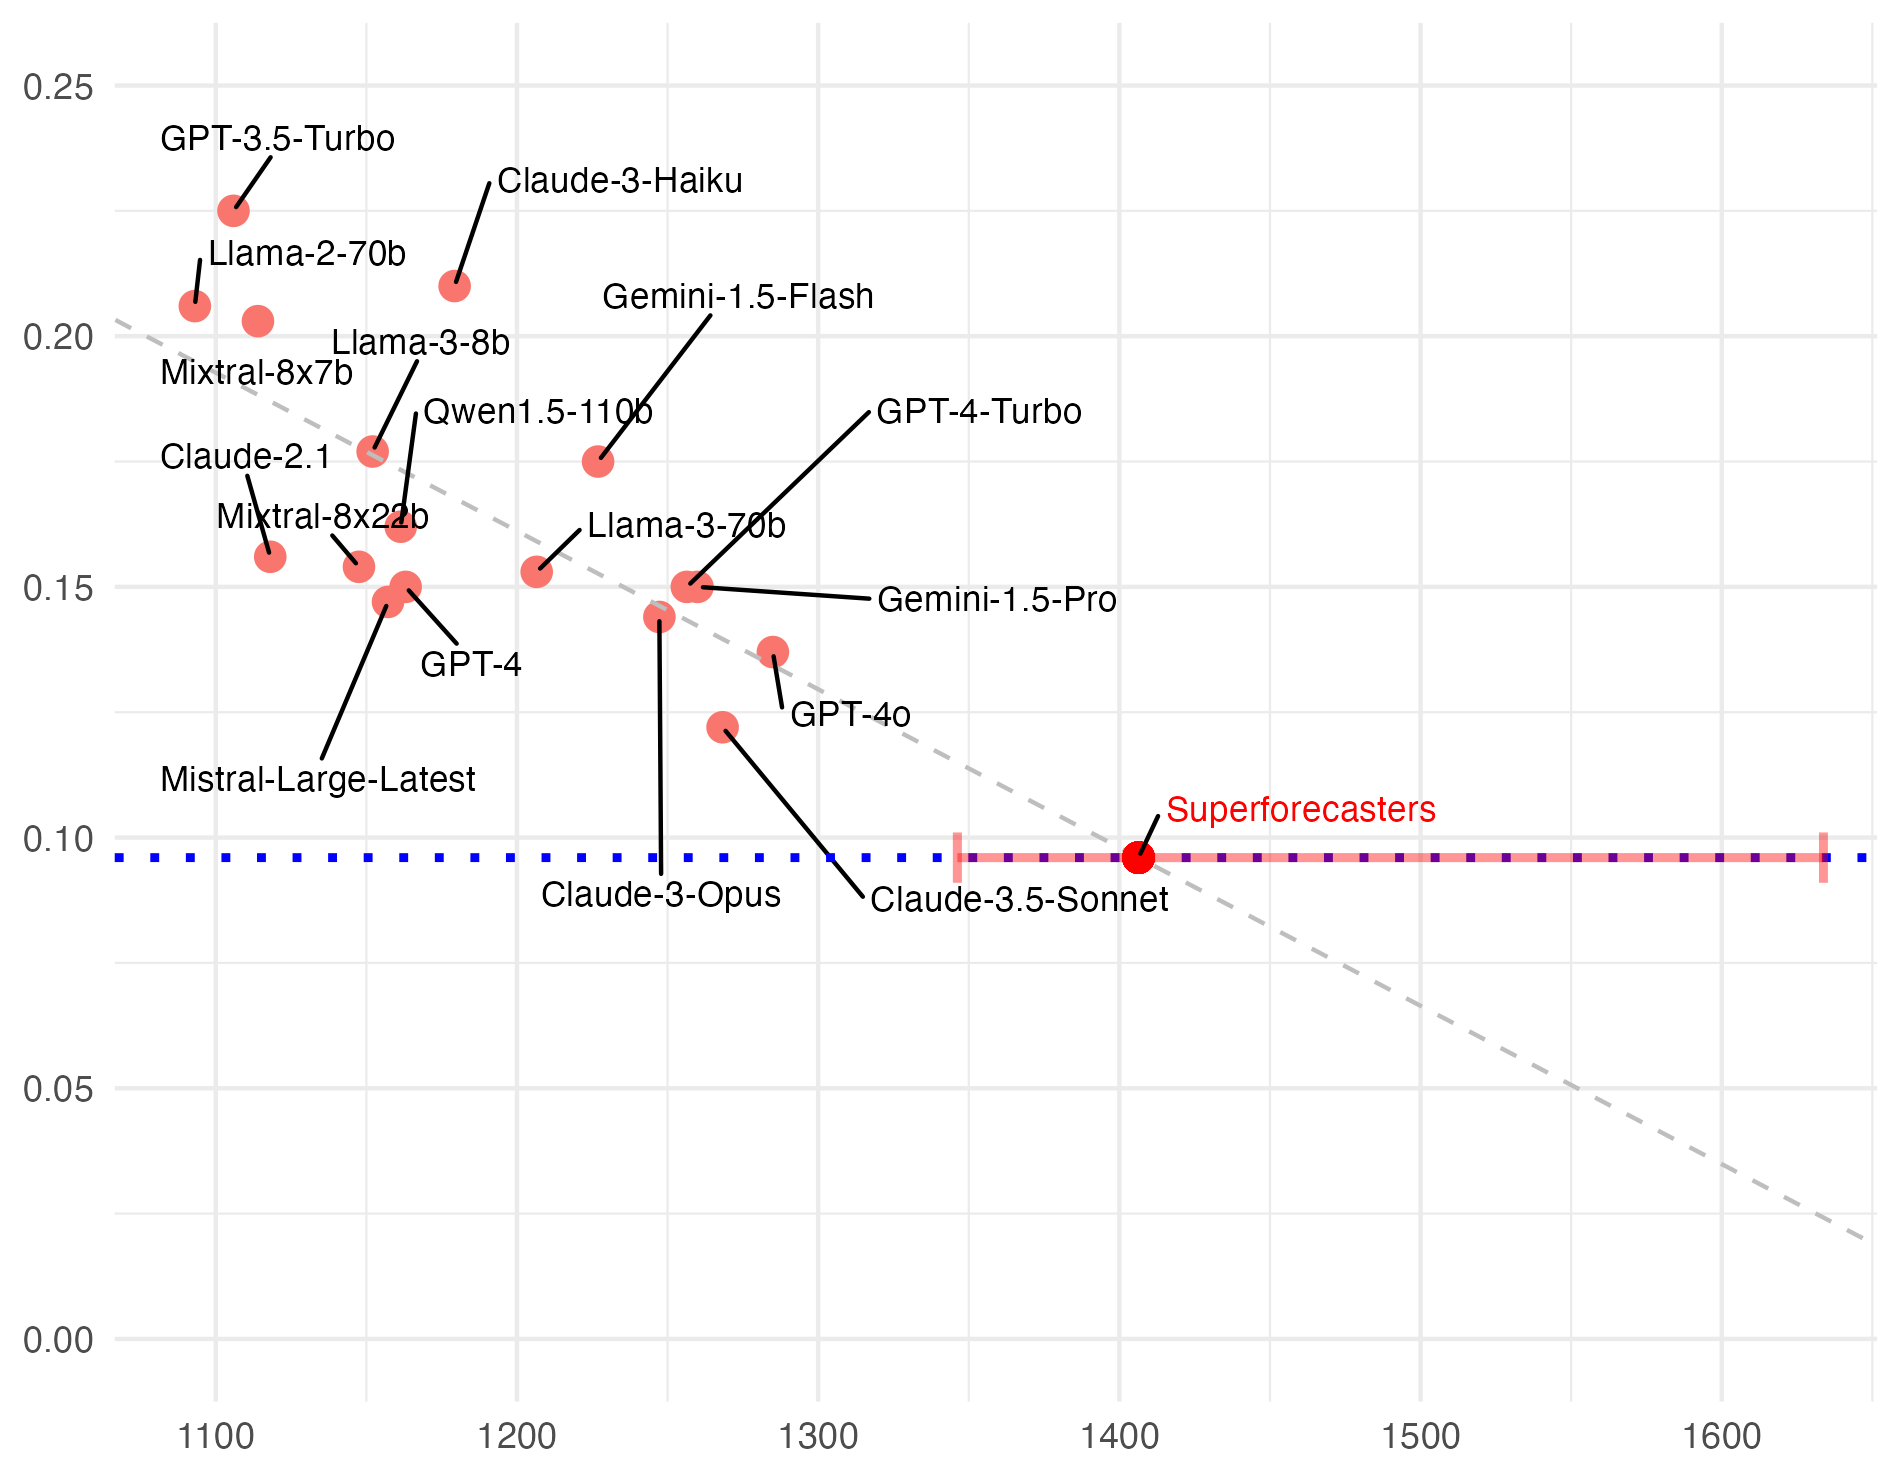
\includegraphics[width=\textwidth]{../arena_v_overall.png}
            };
            \begin{scope}[x={(image.south east)},y={(image.north west)}]
                % Add x-axis label
                \node[below,scale=0.8] at (0.5,0) {Chatbot Arena score (higher is better)};
                \node[rotate=90,left,scale=0.8] at (-0.02,.85) {Brier score (lower is better)};
            \end{scope}
        \end{tikzpicture}
    \end{subfigure}%
    \hspace*{1em}%
    \begin{subfigure}[t]{0.475\textwidth}
        \centering
        \begin{tikzpicture}
            \node[anchor=south west,inner sep=0] (image) at (0,0) {
                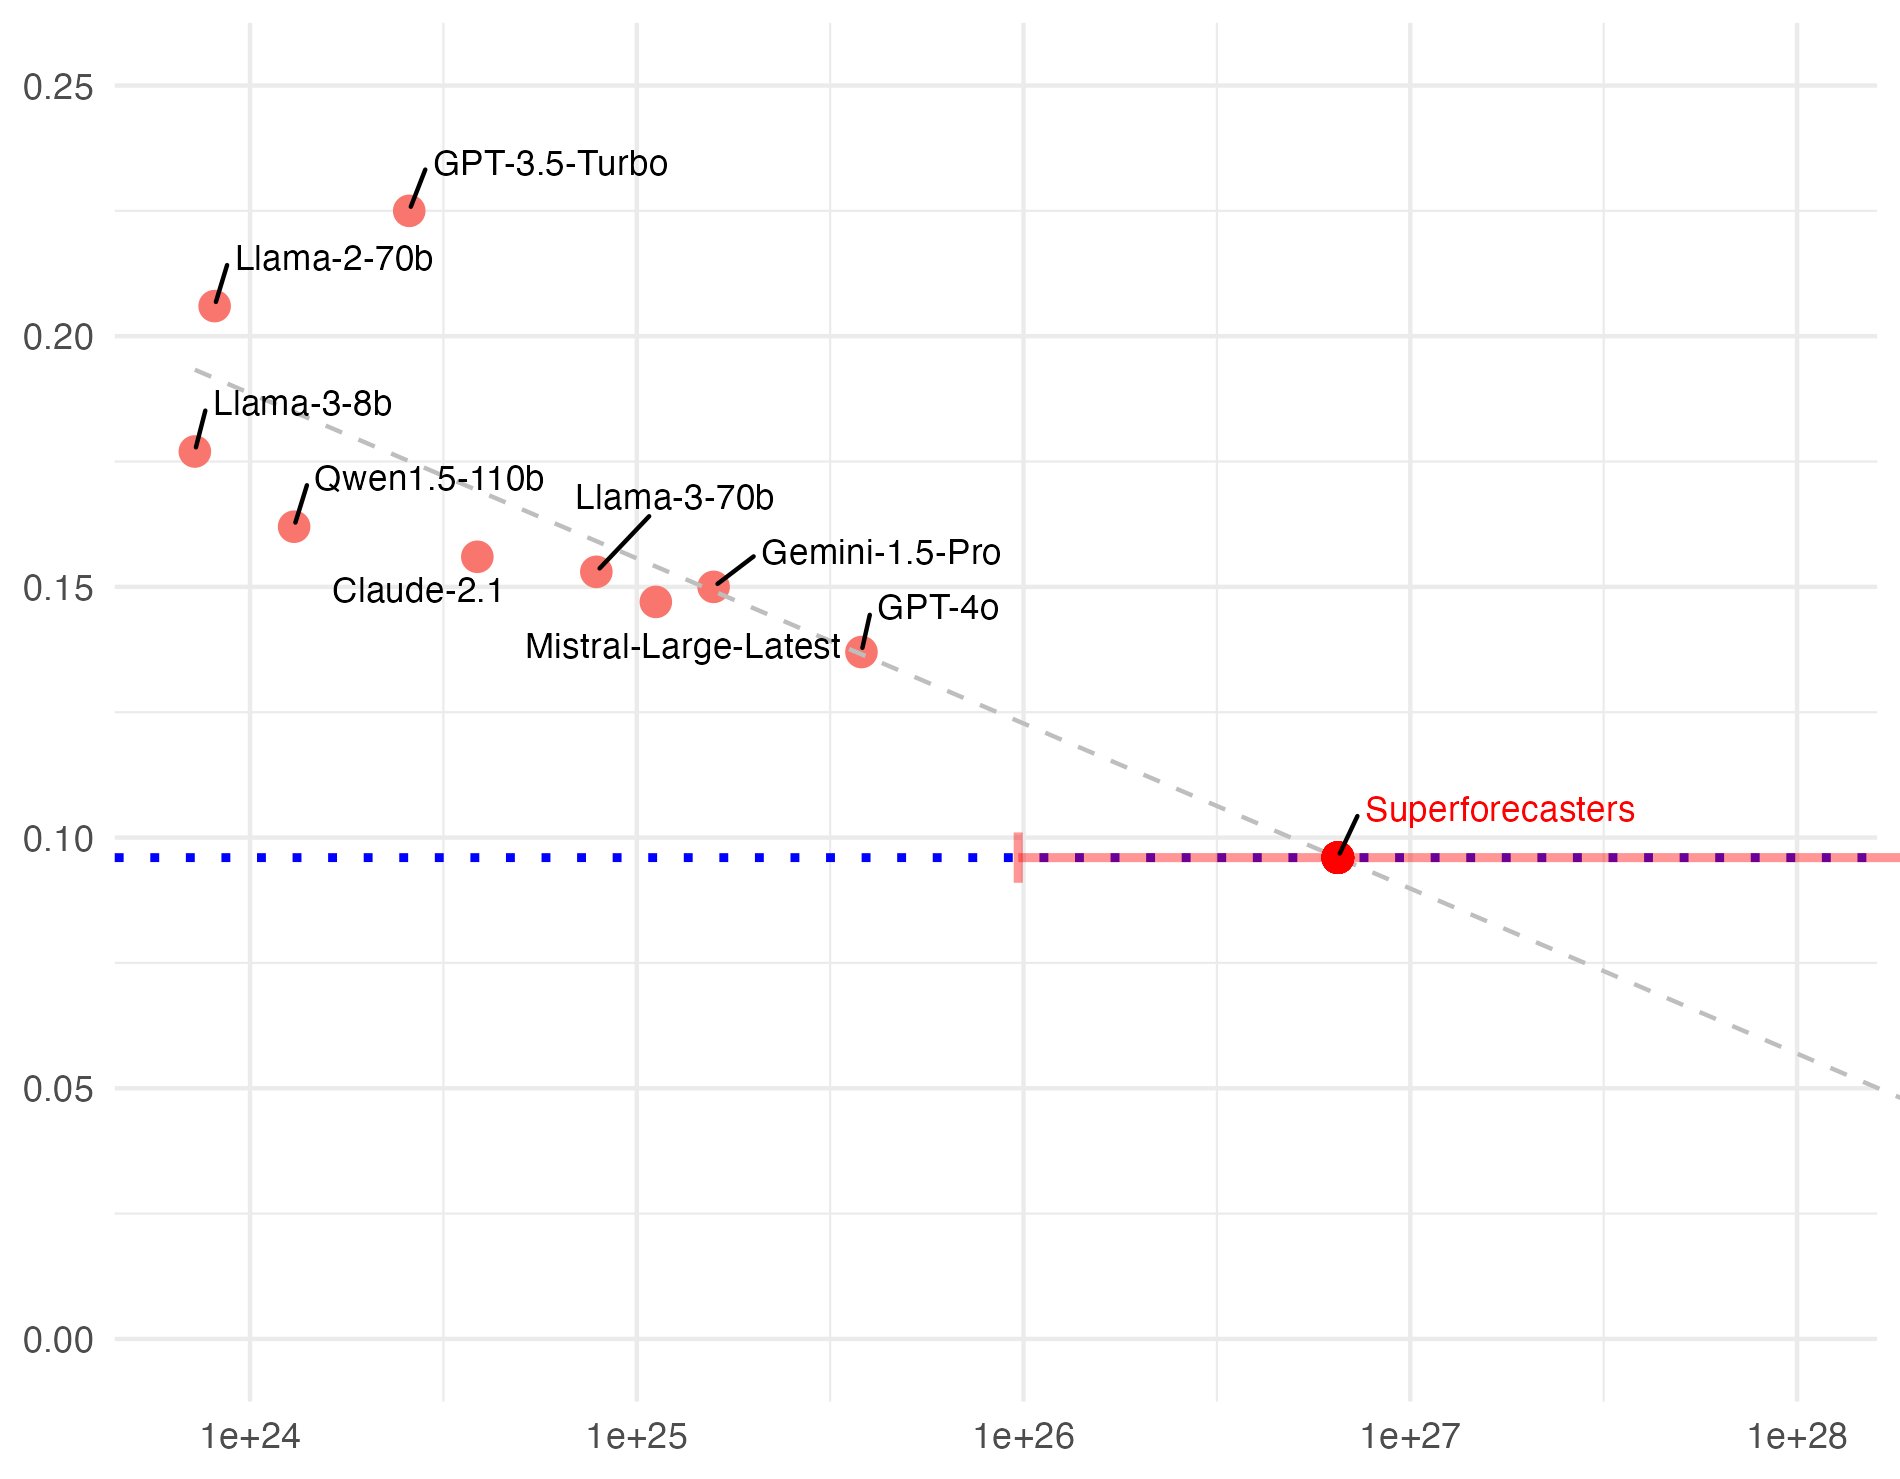
\includegraphics[width=\textwidth]{../tc_v_overall.png}
            };
            \begin{scope}[x={(image.south east)},y={(image.north west)}]
                % Add x-axis label
                \node[below,scale=0.8] at (0.5,0) {Log training compute (FLOP)};
                \node[rotate=90,left,scale=0.8] at (-0.02,.85) {Brier score (lower is better)};
            \end{scope}
        \end{tikzpicture}
    \end{subfigure}
    \end{minipage}
\end{figure}

\end{frame}


\begin{frame}
  \begin{center}
    \vfill
    {\LARGE Contact us to benchmark your model!}
    \vfill
    {\LARGE \texttt{forecastbench@forecastingresearch.org}}
    \vfill
    {\LARGE \href{https://www.forecastbench.org/}{\texttt{https://www.forecastbench.org}}}
    \vfill
  \end{center}
  \vfill
  \begin{columns}[T]
    \column{0.2\textwidth}
    \column{0.09\textwidth}

    \ccbysa
    \column{0.71\textwidth}
    \tiny
    Copyright © 2024-2025 Forecasting Research Institute \\
    License: \href{http://creativecommons.org/licenses/by-sa/4.0/}{Creative
      Commons Attribution-ShareAlike 4.0}
  \end{columns}
\end{frame}

\end{document}
